% this file is called up by thesis.tex
% content in this file will be fed into the main document
\chapter{Evolutionary Algorithms combined with Knowledge Based Systems} % top level followed by section, subsection
%: ----------------------- paths to graphics ------------------------

% change according to folder and file names
\ifpdf
    \graphicspath{{2/figures/PNG/}{2/figures/PDF/}{2/figures/}}
\else
    \graphicspath{{2/figures/EPS/}{2/figures/}}
\fi

%: ----------------------- contents from here ------------------------

\begin{flushright}
Life results from the non-random survival 
\linebreak
of randomly varying replicators.
\linebreak
Richard Dawkins 
\end{flushright}
\section{Evolutionary Algorithms}
Evolutionary Algorithms (EAs) are an interdisciplinary research topic with relation to biology, artificial intelligence, numerical optimization and engineering \cite{Back1996}. EAs belong to the population based, stochastic optimization methods and mimic Darwin's theory of evolution on the origin of species \cite{Darwin}. 

EAs have been  used in solving optimization problems at the beginning of the 60s simultaneously in the form of evolutionary strategies \cite{Rechenberg} and evolutionary programming \cite{Fogel}. An other variation of EA is genetic algorithm (cite Frase, Goldberg) which was proposed as a tool for simulating the evolution of species. Genetic programming (cite Koza J) on the other hand is a extreme variation of EA in which evolution operators create programmes aiming at the solution of the problem in hand. The classification of EAs in the aforementioned variants has lately fallen in disperse since the majority of modern algorithms borrows characteristics of all of them, thus placing everything under the general category of evolutionary algorithms.     

EAs main characteristics are the population based evolution and the fact that the inheritance of genotype is based on probabilistic criteria and the decisions made based upon a fitness function quantifying the ability of each individual to survive in a given environment, where environment is a function of the optimization objectives. 

Evolution, from each generation to the next, fig~\ref{EA}, is achieved with the use of evolution operators, inspired from Darwin's theory of evolution, namely recombination, elitism, mutation, etc. The need to evaluate all the individuals of the population, in order to assign individual fitness values according to the environment, is the main draw-back of EAs when dealing with industrial case engineering optimization problems due to the high computational cost of each individual fitness-assignment yielding a collectively extremely high computational coast for each optimization. An efficient way to reduce the computational cost is the employment of metamodels (cite). Metamodels are either pattern recognition tools that can recognise if the individual genotype (pattern) is promising or not (cite), or interpolation/approximation tools that can approximate/predict the individual's fitness value (cite).     

\figuremacroW{EA}{EA schematic representation }{This figure shows a schematic representation of the evolutionary algorithm population cycle. Each population is derived by the previous one via genetic operators i.e. parent selection, crossover and mutation }{0.8}

Optimization problems that concern this thesis can be formulated as:
\begin{align} 
   &min ~ F(x)=(f_1(x),f_1(x),...,f_M(x))\in \Re^{M} \nonumber \\
   &\mbox{subject to} ~ c_k(x)\leq d_k ~ k =1,K
\label{OptimIN}
\end{align}
where $x\in X \!\leq\! \Re^{N}$ is the design vector and $X$ the design space. If equality constraints are enforced $ c^*(x)=d^* $, they can be transformed into inequality constraints $ c(x)=\Vert c^*(x)-d^*\Vert \leq d $ where $ d \in \Re $ a very small number.  Problem \ref{OptimIN} becomes a multi-objective optimization problem if $M \!> \!1$, in such case the sense of Pareto dominance (cite) is used to define each individuals fitness. 
 
\subsection{Generalised Evolutionary Algorithm}

Each generation $g$ of a generalised EA is defined by three populations. The offspring $P_{\lambda}^g$ population, the parent $P_{\mu}^g$ population and the elite $P_{e}^g$ population. $P_{e}^g$ contains the current best pareto front approximation. Depending on the coating (binary, binary grey or real) the correct evolution operators should be applied. 

\begin{itemize}
\item[]{\bf step 1:}  (Initialization), $g=0$, $P_{\mu}^0=0$ and $P_{\mu}^0=0$. All members of $P_{\lambda}^1$ are initialized using a, uniform within design bounds,  pseudo random number generator.  
\item[]{\bf step 2:}  (Evaluation), for every member of $P_{\lambda}^g$ the vector $F(x) \in \Re^{M} $ is evaluated. In full scale engineering problems evaluation is the most computationally demanding step.
\item[]{\bf step 3:}  (Fitness assignment), for every member of the generations population $x \in P^g$ where $P^g = P_{\lambda}^g \cup P_{\mu}^g \cup P_{e}^g$ a scalar fitness $f(x)$ value is assigned. In single objective problems $f(x)=F_1(x)$. On the other hand for multi-objective problems a variety of methods that compute the individual's fitness based on the pareto dominance of $F(x)$ and distance on either design or objectives space.
\item[]{\bf step 4:}  (Elite selection), from population $P^*$ where $P^*=P_{\lambda}^g \cup P_{e}^{g-1}$ the $e^*$ not dominated individuals are selected to be $P_e^g$. If $e^* > e$ a dilution operator is applied to remove $e^* - e$ neighbouring individuals.     
\item[]{\bf step 5:}  (Elitism), a number of user specified elite individuals replace the worst members of $P_{\lambda}^g$.  
\item[]{\bf step 6:}  (Parent selection), Parent population is selected from $P_{\mu}^{g-1}$ , $P_{\lambda}^g$ taking into account the maximum generations limit  $k$ for each parent. $P_{\mu}^{g}=S(P_{\mu}^{g-1},P_{\lambda}^g,k)$ 
\item[]{\bf step 7:}  (Crossover), the first for the creation of $P_{\lambda}^{g+1}$ from $P_{\mu}^{g}$ is the application of the crossover operator. Crossover is the process of combining the genotype of $n$ parents to create one offspring. $P_{\lambda}^{'g+1} = C(P_{\mu}^{g})$. 
\item[]{\bf step 8:}  (Mutation), the second step for the creation of $P_{\lambda}^{g+1}$ is the application of mutation operator. Mutation is the process that randomly changes one part of an individuals genotype. $P_{\lambda}^{g+1} = M(P_{\lambda}^{'g+1})$
\item[]{\bf step 9:}  (Finalise criteria check)
\end{itemize}
In the rest of this thesis an evolutionary algorithm with $\mu$ parents and $\lambda$ offspring will be referred to as EA($\mu,\lambda$)   

\begin{table}[htdp]
\centering
\begin{tabular}{lr} 
\hline
\hline
number of objectives & M\\
number of design variables & N\\
number of constraints   & K\\
\hline
candidate solution   & x\\
objectives vector  & F\\
constraints vector  & C\\
fitness values & f\\
\hline
\hline
\end{tabular}
\caption[GEA nomenclature]{GEA nomenclature}
\label{GEA nomenclature} 
\end{table}
\subsection{Genetic operators}
\paragraph{Crossover}
Since the original formulation of GAs (cite holland) there has been numerous discussions about the merits of crossover as a search mechanism. In its majority the research work inspired by this discussions was concentrated on contrasting the behaviour of algorithms employing crossover as one of there reproduction operators as opposed to mutation only based ones. 
In general, although crossover is much less effective at resisting the tendency of selection pressure towards population convergence - as soon as all the population has converged to the same value, say a local optima, crossover (unlike mutation) is unable to retrieve the lost diversity (cite Schaffer Morishima 1987). Crossover though, until the population is almost entirely converged, has a greater ability to construct higher order schemata from good lower order ones, also known as the building block hypothesis (cite Spears 1992).         
Simply put, crossover is the evolution operator that takes advantage of the Schema theorem based building block hypothesis in order to increase the probability of offspring which are fitter than their parents.    

These issues have in fact been studied many decades prior of the invention of modern computers and genetic algorithms. Sexual reproduction in particular and what benefits it offers have long been studied by evolutionary biologist (cite biobook .. Maynard-Smith or Szathmary). 

From the point of view of the "selfish gene" (cite Dawkings), "parthenogenesis" (asexual reproduction) would initially appear more advantageous, since all of an organism's genes would survive to the next generation (saving mutation). In that sense it is expected from a gene that prompts parthenogenesis to dominate fast over a sexually reproductive population, that gene could arise through a mutation. However when finite population is taken into account Muller's Ratchet effects come into play (cite Muller). Muller's ratchet is the process by which the genomes of an asexual population accumulate deleterious mutations in an irreversible manner. By contrast if crossover is allowed Muller's ratchet can be avoided, this has led to the view of crossover as a gene repair mechanism (cite Maynard-Smith 1978). Also a similar to the Building block hypothesis reasoning is used by biologist witch shows that in populations in changing environment crossover leads to faster accumulation and combination of successful mutations (cite Fisher, 1930), this is also known as "hybrid vigour".            

\subparagraph{Schema theorem and building block hypothesis}
The theoretical analysis and thinking about GAs has been dominated from two related concepts, that of Schemata and Building Blocks. A schema can be seen as a hyper-plane in the search space, good shemata being the hyper-planes that concentrate high fitness individuals. A common presentation of the shemata concept is made for binary alphabet via the addition of a third symbol, the "don't care" symbol $\#$. For a five digit problem i.e. the $11\#\#\#$ shcema is a hyperplane in the design space defined by $1$ in the first two places of the string. The total number of strings that belong to this hyperplane is said to be examples of this schema (in this case $2^3 = 8$). 

Two features are generally used to describe a schema, the order of the schema (number of digits in the schema witch are not $\#$) and the defining length (the distance between the outermost defined digits). Thus a schema $H=1\#\#0\#1\#0$  has order $o(H)=4$ and defining length $d(H)=8$.

The probability of a schema to be selected ($p_s$) depends on the fitness of the individual that contains it, based on the parent selection operator. The probability of disrupting a schema during crossover ($p_d^c$) depends on one hand by the type of the crossover operator and the defining length, for one point crossover i.e. the schema will be disrupted if the crossover point falls between the ends witch happens with probability $ d(H)/l-1 $. Similarly the probability of disrupting a schema from mutation ($p_d^m$) depends its order  $o(H)$.

The proportion $m(H)$ of individuals containing the schema $H$ at subsequent generations is therefore:
\begin{eqnarray}
   m(H,g+1)\geq m(H,g)\times p_s \times (1-p_d^c-p_d^m) 
   \label{Schema} 
\end{eqnarray}

Related to the schema theorem is the Building Block Hypothesis (cite Goldberg,1989). GAs according to the Building Block Hypothesis work by discovering lower order schemata of high fitness, the so called building blocks, and combine them via crossover to create new potentially fit schemata of higher order. This process is frequently referred to as mixing.

\subparagraph{Offspring probability distribution} 
A convenient and intuitive way to demonstrate and analyse how crossover algorithms work is via plotting the probability distribution of offspring on the design space based on the current parents. The Offspring probability distribution essentially shows for each point of the design space the probability of an offspring to appear based on its parents.

\begin{eqnarray}
	P(\overrightarrow{x})=f(\overrightarrow{x_{p1}},\overrightarrow{x_{p2}},C())    
    \label{prob_eq} 
\end{eqnarray}


Two typical examples of offspring probability distributions are presented in fig. \ref{Crossover}
%\figuremacroW{Crossover}{}{Typical Offspring probability distribution of a two parent ($P1\& P2$) crossover for a one-dimensional problem.}{0.8}


\begin{figure}[h!]
\begin{minipage}[b]{0.5\linewidth}
 \centering
 \resizebox*{7.0cm}{!}{\includegraphics{Crossover.eps}}
\end{minipage}
\begin{minipage}[b]{0.5\linewidth}
 \centering
 \resizebox*{7.0cm}{!}{\includegraphics{Crossover2.eps}}
\end{minipage}
\caption{Typical Offspring probability distribution of a two parent ($P1\& P2$) crossover for a one-dimensional problem. The two distributions correspond to two different crossover operators.}
\label{Crossover}
\end{figure}
%\subsection{Simulated binary crossover (SBX)}
\paragraph{Mutation}
A broad distinction can be drawn between the two types of reproductive operators according to the number of individuals that are taken as input. I this thesis the term mutation operator is used for those that act on a single individual producing one individual as output as opposed to crossover that that acts on more than one individual to produce a single offspring. 
  
The purpose of mutation in an EA scheme is to introduce and preserve diversity in the population. Thus mutation prevents the population of chromosomes from becoming too similar to each other, thus slowing or even stopping/stagnating the evolution.    

\subparagraph{Offspring probability distribution} 
The offspring probability distribution of the mutation operator is expressed as a function of the distance from the to-be-mutated individual.

\begin{eqnarray}
	P(d)=f(d,M()),~~ d=\sqrt{\sum _{i=1}^N (x_i-x_i^{mut})^2}   
    \label{prob_eq_mut} 
\end{eqnarray}
where $\overrightarrow{x}$ the individual before mutation and $\overrightarrow{x^{mut}}$ after.


\begin{figure}[h!]
\begin{minipage}[b]{0.5\linewidth}
 \centering
 \resizebox*{7.7cm}{!}{\includegraphics{Mutation.eps}}
\end{minipage}
\begin{minipage}[b]{0.5\linewidth}
 \centering
 \resizebox*{7.0cm}{!}{\includegraphics{Mutationb.eps}}
\end{minipage}
\caption{Offspring probability distribution of different types of mutation operators. Left different types of probability distributions, from uniform to $d=d_{Gaussian}^n$. Right same probability distribution types (uniform) with different $d$ range.}
\label{Mutation}
\end{figure}


%\subsection{SOM-based}

\subsection{Multi Objective Evolutionary Algorithm}
Problem \ref{OptimIN} is, in its general form, a constrained multi-objective problem. If a solution $\overrightarrow{x}$ that simultaneously minimizes all objectives then this is the overall solution of \ref{OptimIN}. In case of contradictive objectives though Pareto front optimacy is in use.

\paragraph{Pareto optimacy} Solution $\overrightarrow{x_1}$ dominates solution $\overrightarrow{x_2}$ ($\overrightarrow{x_1}\prec\overrightarrow{x_2}$) if and only if it has better (smaller for minimization problems) or equal value for all objectives and at least one with better value in respect to $\overrightarrow{F(\overrightarrow{x_2})}$.

\begin{eqnarray}
    \overrightarrow{x_1}\prec\overrightarrow{x_2} \Leftrightarrow (\forall _i :  f_i(x_1) \leq f_i(x_2))\wedge (\exists _i : f_i(x_1) < f_i(x_2))
   \label{pareto_eq} 
\end{eqnarray}

\paragraph{Pareto optimal solution} Solution  $\overrightarrow{x_1}$ is a Pareto optimal solution if and only if it is not dominated by any other solution.% Hence the Pareto optimal front is also known as the front of non-dominated solutions.  


\begin{eqnarray}
    \nexists\overrightarrow{x}:\overrightarrow{x}\prec\overrightarrow{x_1}
\end{eqnarray}
 
\figuremacroW{Pareto2}{}{Schematic representation of Pareto optimacy. $\overrightarrow{x_1}$ is a Pareto optimal solution since it is not dominated by any other solution furthermore $\overrightarrow{x_1}$ it self dominates all the solutions located in the grey box.}{0.7}

Assuming that the individuals shown in fig. \ref{Pareto2} is the population of an EA generation, with black points the current Pareto front approximation is noted and with white points all the dominated individuals. Furthermore the aria dominated by $\overrightarrow{x_1}$ is shown in grey, the individuals located in the grey aria are dominated at least by $\overrightarrow{x_1}$. 

\paragraph{Fitness assignment for multi-objective problems.}
Even though for single-objective optimization fitness assignment is equivalent with the individual evaluations ($f(\overrightarrow{x})=F(\overrightarrow{x})$) in multi-objective problems things are different. In multi-objective problems a procedure is needed to reduce the $M$-dimentional vector of objectives $\overrightarrow{F(\overrightarrow{x})}$ into a scalar metric $f(\overrightarrow{x})$ that will represent the individual's fitness. 

\begin{eqnarray}
    f(\overrightarrow{x})=f(\overrightarrow{F(\overrightarrow{x}))} :\Re ^M \rightarrow \Re ^1 
\end{eqnarray}

There is a lot of different algorithms proposed in literature that offer this ability. A complete review of literature on the subject can be found in cite(K 69,70,71). Furthermore the Strength Pareto Evolutionary Algorithm II (SPEA II), that is used in this thesis, will be presented cite (K 73,74).

\paragraph{SPEA II}
is an improvement over SPEA cite(K 66). The improvements consist on the additional information about the number of dominated, by the in fitness evaluation individual, individuals as well as the one that dominate it. The use of density information additionally helps on the better distribution of the individuals on the Pareto front (traditional SPEA had a bias of favouring the individuals located in the middle of the Pareto). 

\subparagraph{Strength} is defined in SPEAII algorithm as the sum of the dominated      by the in fitness evaluation individual, individuals divided by the total number of the individuals in the population.  


\subparagraph{SPEA II algorithm}

\begin{itemize}
\item[]{\bf step 1:}  (Strength calculation), the strength of every member of the population is computed. 
\begin{eqnarray}
	\nonumber
	\forall i \in P = P_{\lambda}^g \cup P_{\mu}^g \cup P_{e}^g  
\end{eqnarray}
\begin{eqnarray}
	S_i = \frac{\sum(j : j \in P \wedge i \prec j)} {\sum P} 
\end{eqnarray}

\item[]{\bf step 2:}  (Density calculation), the density metric is calculated for every member of the population as the distance between it and its closest neighbour.latex equation no number

\begin{eqnarray}
	D_i = \frac{1} {d_i+2} 
\end{eqnarray}
where
\begin{eqnarray}
	\nonumber
	d_i= min (\parallel \overrightarrow{F_i} - \overrightarrow{F_k} \parallel), ~ k \in P  
\end{eqnarray}


\item[]{\bf step 3:}  (f calculation), the fitness value for all the members of the population is calculated as the sum of raw fitness $R_i$ and the density metric.

\begin{eqnarray}
	f_i = R_i+D_i
\end{eqnarray}

where $R_i$ is the sum of the individual strengths of the population members that dominate it.
  
\begin{eqnarray}
	\nonumber
	R_i=\sum _{j \in P \wedge i \prec j}(S_j)  
\end{eqnarray}  
\end{itemize}

\paragraph{Hypervolume indicator}
A quality measure of the Pareto front is needed for the comparison of the different optimization techniques for multi-objective optimization. In this thesis the Hypervolume indicator is chosen for that purpose (cite The Hypervolume Indicator Revisited: On the Design of Pareto-compliant Indicators Via Weighted Integration). Hypervolume indicator assumes that the quality of a pareto front can be quantified in a scalar value, the hypervolume of the dominated by the Pareto front portion of the objective space. 

The hypervolume indicator of a set $A$  and reference point $(b_1,...,b_M)$ is defined as:
\begin{eqnarray}
	I(A)=\int _{(0,...,0}^{(b_1,...,b_M)}a_A(x)dx 
\end{eqnarray}  
where,

\begin{eqnarray}
	\nonumber
	a_A(x) = \left\{ \begin{array}{ll}
    1 & \mbox{if $(A\prec{x})$}\\
    0 & \mbox{else}\end{array} \right.
    ,~x\in A
\end{eqnarray}    


\begin{figure}[h!]
\begin{minipage}[b]{0.5\linewidth}
 \centering
 \resizebox*{6.5cm}{!}{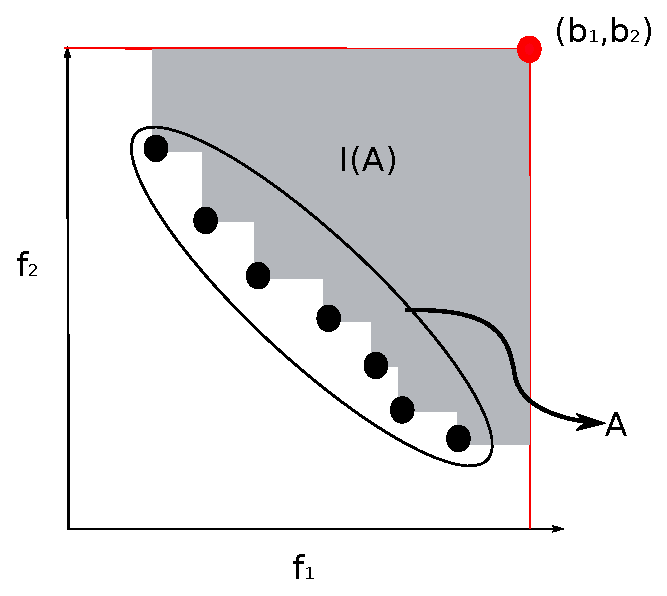
\includegraphics{hyperVol.eps}}
\end{minipage}
\begin{minipage}[b]{0.5\linewidth}
 \centering
 \resizebox*{10.0cm}{!}{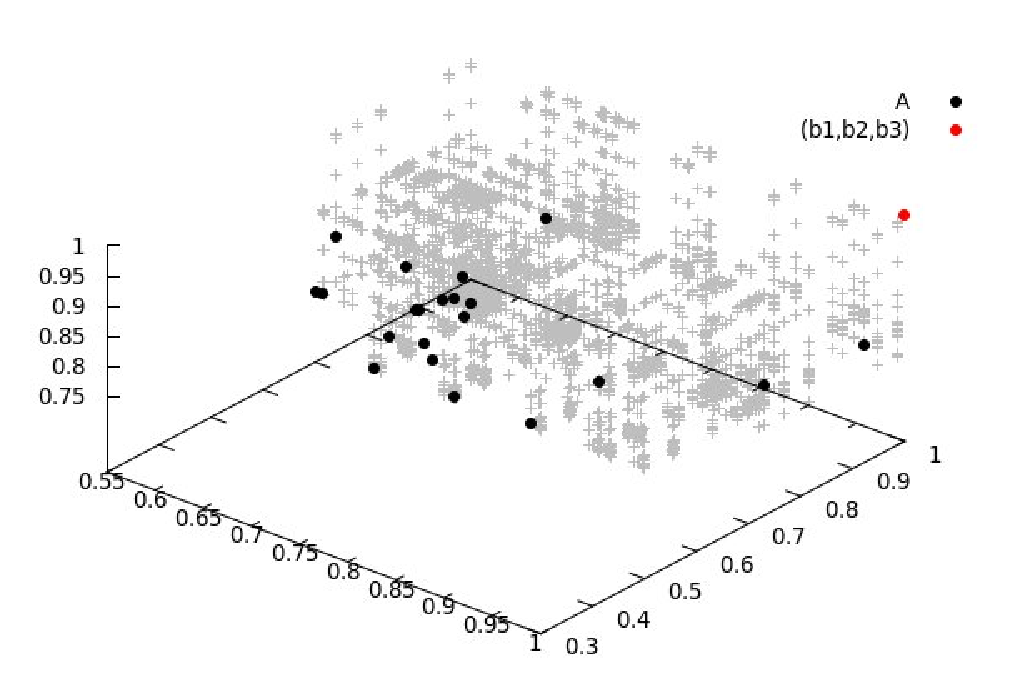
\includegraphics{pareto3d.eps}}
\end{minipage}
\caption{Two dimensional (left) and three dimensional (right) examples of hypervolue indicatror for set $A$. Reference point is $(b_1,...,b_M)$.}
\label{hyperV}
\end{figure}

Hypervolume indicator is the ideal tool to compare efficiency of different multi-objective optimization techniques since to have accurate comparisons the only prerequisite is a reference point (the same for all the for-comparison fronts) that is dominated by all the solutions of all the fronts.   

\subsection{Constrained optimization}
EAs are not inherently build to handle contained optimization problems. In engineering cases though it is usual for a number of constraints to govern the optimization problem in hand. The most common in literature way to deal with constraints in an EA environment is the use of penalty functions (cite K56 K76 K77), assigning evolutionary advantages to the individuals that fulfil the constraints (cite K78), conversion of constraints into objectives (cite K79, K80) and the use of correction operators (cite K81). Complete literature review about the subject can me found in (cite K82 K83).

In this thesis an improved version of the penalty functions technique is in use. In the traditional penalty functions technique EA takes into account the constraints by  incrementing penalties (relative to the magnitude of the constraint violation) on the objectives. For each constraint except of the hart limit ($d$, the value of the constraint quantity that has to be respected) additionally a relaxed limit is introduced $d_k^*$. As soon as an individual violates the relaxed limit of one of the objectives ($c_k>d_k^*$)it suffers death penalty ($\overrightarrow{F} = \infty$). If the individual violates one, or more, of the constraints ($c_k>d_k^*$) but none of the relaxed limits a vector of penalised objectives ($\overrightarrow{F^P}=\overrightarrow{F^P}(\overrightarrow{F},\overrightarrow{C},\overrightarrow{A},\overrightarrow{a})$), where $\overrightarrow{A},\overrightarrow{a} \in \Re$ penalization control vectors, is constructed. 

\begin{eqnarray}
	F_i^P=F_i+A_i \prod _{k=1}^K{\left\{ \begin{array}{ll}
    exp(a_k\frac{c_k(x)-d_k}{d_k^* -d_k}) & ~~,c_k(x)>d_k\\
    1 & ~~,c_k(x)\leq d_k\end{array} \right. }
    \label{penal}
\end{eqnarray}  

In order to accommodate the influence of the constraints in the evolutionary operators the fitness assignment step (here SPEAII) uses instead of objectives vector the penalised objectives vector.  
\begin{eqnarray}
	f(\overrightarrow{x})=f(\overrightarrow{F^p}(\overrightarrow{x}))
\end{eqnarray}  

In case of multi-objective optimization subject to multiple constraints the above technique has the drawback of creating sharp edges (steps) on the $f(\overrightarrow{x})$ near the constrain borders (fig .\ref{fit1}). Coupled with that comes the biased penalization alongside the border (some regions of the border are penalised harder than others, with respect to the distance form it). The biased penalization its self influences the probability of the individuals close to the constraint border to be selected to undergo evolution operators thus creating a bias in the ability of the EA to search in the vicinity of the boarder. Given that for a big portion of the engineering cases the optimum is located near the constrain border the aforementioned bias can result in significantly biased results.


\begin{figure}[h!]
\begin{minipage}[b]{1.0\linewidth}
 \centering
 \resizebox*{15cm}{!}{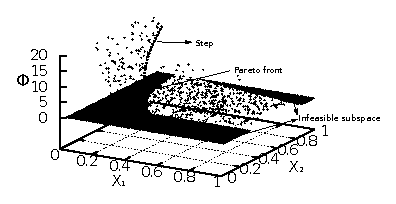
\includegraphics{fit_old.eps}}
\end{minipage}
\caption{Fitness plot for 1000 randomly chosen individuals over the two-dimensional design space of a two objective constraint optimization problem using the traditional penalization method (eq.\ref{penal}) to handle the constraints and SPEAII as fitness assignment algorithm. Constraint region is noted with grey.}
\label{fit1}
\end{figure}

To overcome this a decision was made to move the application of penalty from the objective vector directly to the fitness value. So fitness evaluation takes place as if the problem was without constraints ($f(\overrightarrow{x})=f(\overrightarrow{F}(\overrightarrow{x}))$) and the penalization equation (eq.\ref{penal}) is transformed into; 


\begin{eqnarray}
	f(\overrightarrow{x})=f(\overrightarrow{x})+ \prod _{k=1}^K{\left\{ 				\begin{array}{ll}
    exp(a_k\frac{c_k(x)-d_k}{d_k^* -d_k}) & ~~,c_k(x)>d_k\\
    1 & ~~,c_k(x)\leq d_k\end{array} \right. }
    \label{penal2}
\end{eqnarray}  

Where in comparison with (eq.\ref{penal}) the control vector $\overrightarrow{A}$ vanishes and $\overrightarrow{a}$ remains to control the penalization intensity for each individual constraint.

\begin{figure}[h!]
\begin{minipage}[b]{1.0\linewidth}
 \centering
 \resizebox*{15cm}{!}{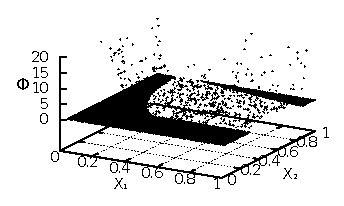
\includegraphics{fit_new.eps}}
\end{minipage}
\caption{Fitness plot for the same 1000 individuals of fig.\ref{fit1} of the same optimization problem but this time using the adapted penalization formulation (eq.\ref{penal2}) . Fitness value increases (minimization problem) exponentially as the individuals move further in the constraint region.}
\label{fit2}
\end{figure}


%\begin{figure}[h!]
%\begin{minipage}[b]{1.0\linewidth}
% \centering
% \resizebox*{15cm}{!}{\includegraphics{fit_new_in.eps}}
%\end{minipage}
%\caption{Two dimensional (left) and three dimensional (right) examples of hypervolue indicatror for set $A$. Reference point is $(b_1,...,b_M)$.}
%\label{fit3}
%\end{figure}





%\subsection{Distributed Evolutionary Algorithm}

\subsection{Hierarchical Evolutionary Algorithm}
Typically in engineering design a number of tools with different fidelity and cost (computational and/or economic) are available and used in different steps of the design procedure (fig.\ref{HMAEA} right). Relatively fast low fatality tools are used in the initial stages of the design in order to efficiently scan the design space and high fatality slow (and/or expensive with respect to licensed software or laboratory time) tools are used for the latter steps of design for fine-tuning. In case of turbo-machinery design, for example, a potential code can be used as a low fidelity tool followed by dense or coarse grid Euler codes, Navier-Stokes codes for a single flow passage or the full machine and finally actual laboratory test and adaptation cycles.    


\begin{figure}[h!]
\begin{minipage}[b]{1.0\linewidth}
 \centering
 \resizebox*{13cm}{!}{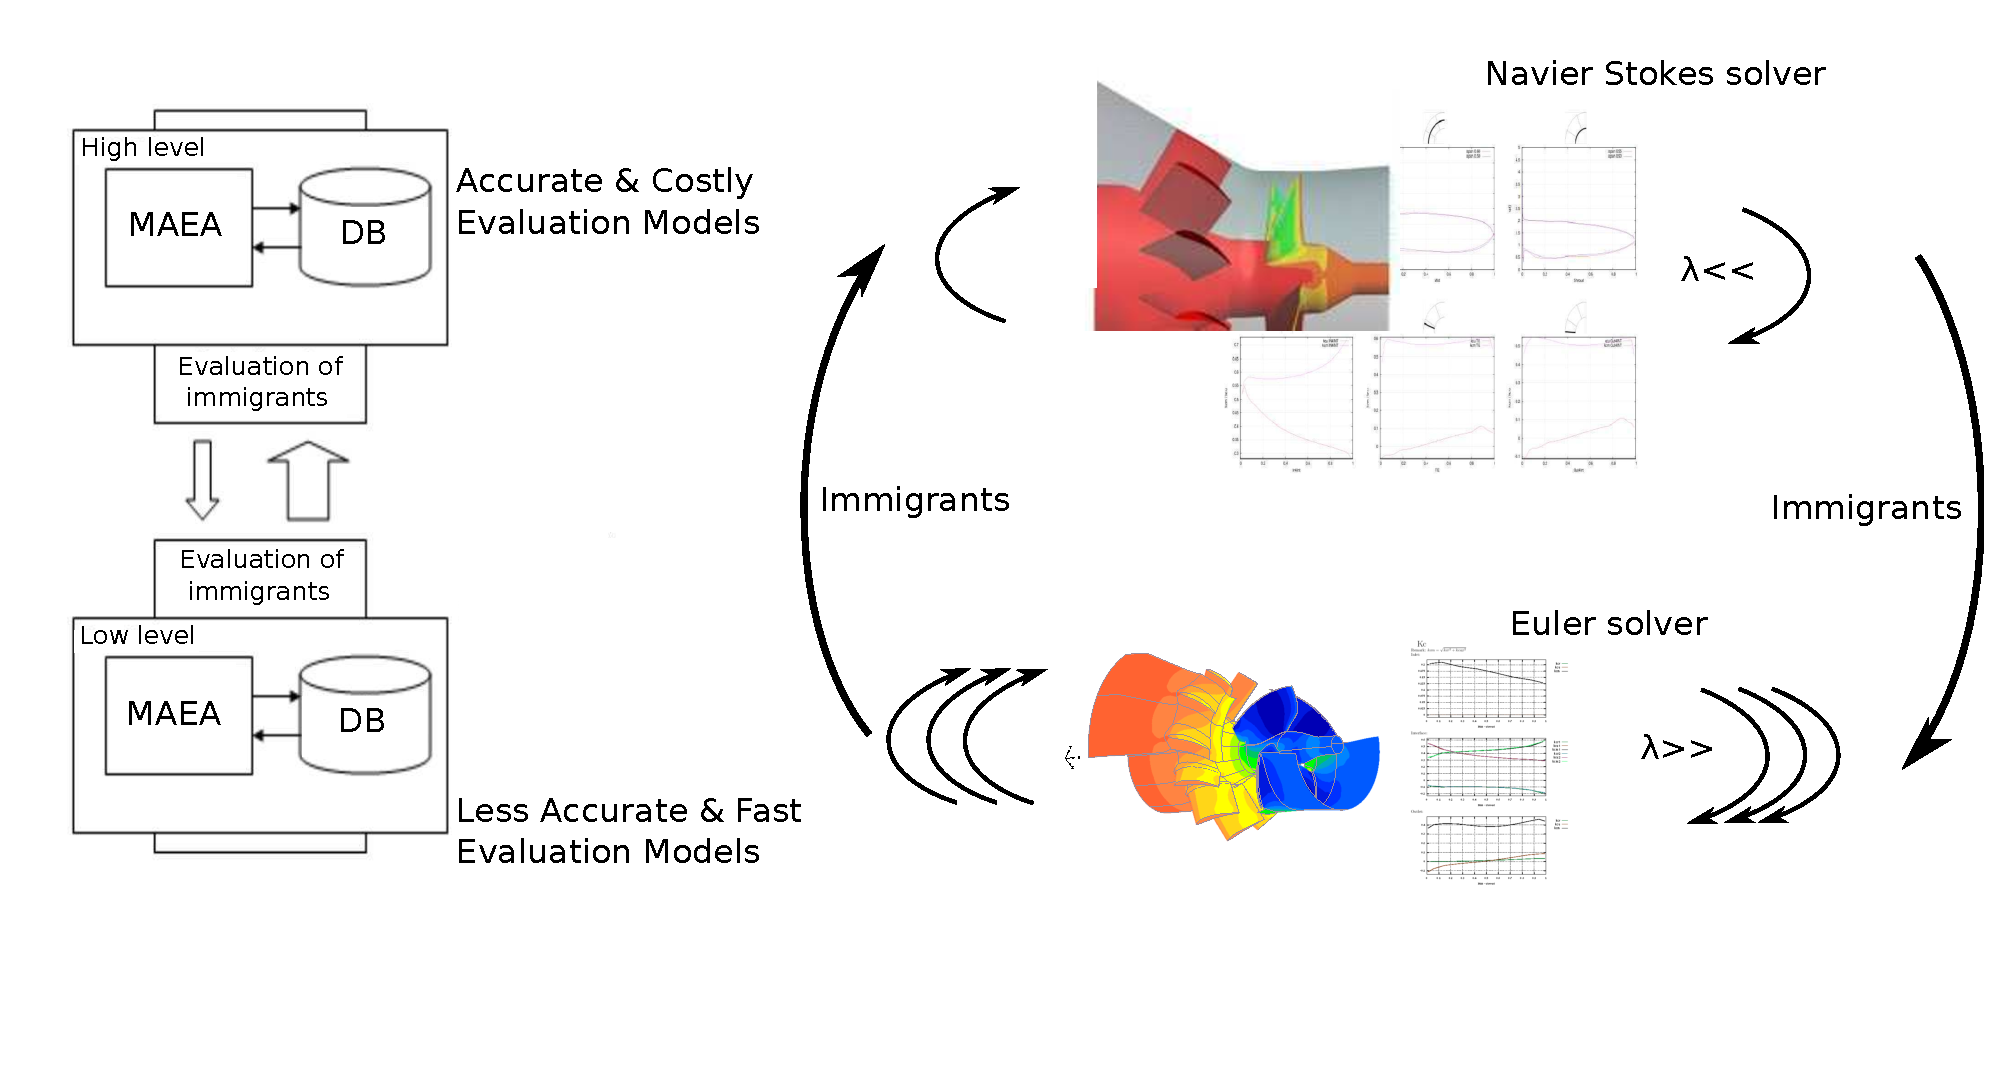
\includegraphics{handmade.eps}}
\end{minipage}
\caption{Left, schematic representation of a two level HMAEA (Hierarchical metamodel assisted evolutionary algorithm). High level is associated with the expensive and accurate tool and lower level with the cheap but not so accurate tool. Communication between the two level is possible in both directions including re-evaluation with the receiving levels evaluation tool. Right, example of two level design procedure as used in industry. A relatively big number of designs is evaluated with the Euler solver once a good design is located it is evaluated with the Navier-Stokes solver. Possible faults are identified, targets for the lower level are updated, that would result in the  elimination of the aforementioned faults, bye experienced designers.}
\label{HMAEA}
\end{figure} 
 
In order to exploit the availability of this tools Hierarchical evolutionary algorithms (HEA) where devised (cite Kampolis + papers). HEA are enhanced EA variants which utilise a number of evolution Levels, each level assigned a different evaluation tool (fig.\ref{HMAEA} left). This multilevel search mechanism splits the computational burden among the levels. On the lower levels, a low cost exploration of the search space is carried out through global search methods, less demanding or less accurate evaluation tools or by even using reduced design variable sets, etc. On the other hand the higher levels undertake the fine-tuning part of the design procedure through denser parameterization, more accurate evaluation tools and/or stochastic or deterministic search methods. These levels mainly serve to refine immigrants from the lower levels. Intercommunication and two-way migrations of individuals between adjacent levels are necessary. The number of levels, the frequency of migration and the number of immigrants are user-defined parameters.

\subsection{Metamodel assisted Evolutionary Algorithm}

Solving engineering optimization problems using EAs typically involves costly evaluation tools (such as CFD tools to numerically predict flows in or around complex 3D geometries in case of turbo-machinery). This may become very computationally demanding because many candidate solutions must be evaluated before reaching the optimal solution (SOO) or solutions (MOO). The extensive, smart use of low-cost surrogate evaluation models (often referred to as "metamodels") during the optimization decreases substantially the number of calls to the computationally expensive, problem-specific evaluation code (CFD) making EAs a viable tool that can routinely be used to solve large-scale industrial optimization problems, with affordable wall clock time. Literature surveys on the use of metamodels within EAs can be found in papers \cite{LTT_2_020,Jin2002,LTT_2_027} or books \cite{KEANEbook}.


Polynomial regression, artificial neural networks, Gaussian processes etc. have all been used as metamodels.  Schemes based on different interactions between the metamodel and the problem-specific evaluation tool have been published. Hereafter, all of them will be referred to as MAEAs. This thesis uses the MAEA presented in \cite{LTT_2_018} (SOO) and \cite{LTT_2_029} (MOO). 

For all but the first few generations, the metamodels are used to pre-evaluate the current population. Based on the outcome of approximate pre-evaluations, a few most promising individuals are identified and these solely undergo evaluation on the problem-specific evaluation tool to compute their "exact" objective function value(s), before proceeding to the next generation. The $(\mu,\lambda)$ MAEA used herein is sketched in fig.~\ref{MAEA}.


\begin{figure}[h!]
\centering
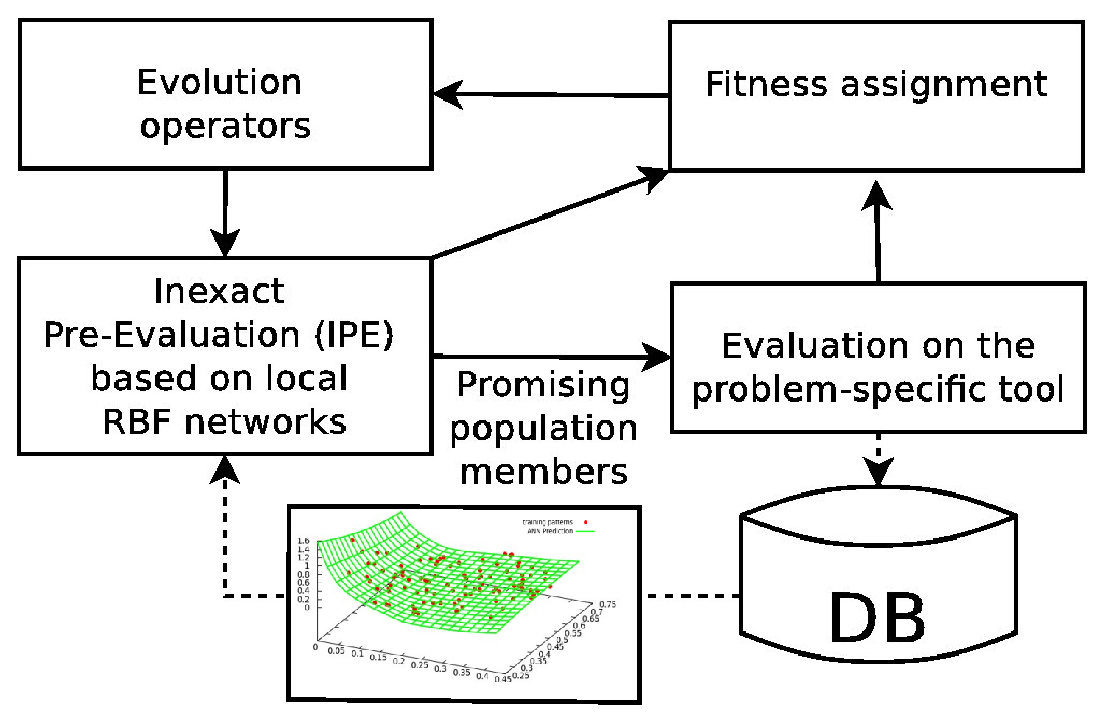
\includegraphics[width=90mm]{MAEA.eps} 
\caption{Schematic representation of the MAEA (namely the variant using on-line trained metamodels) this paper relies on. The loop corresponds to a single EA generation. The so-called inexact pre-evaluation (IPE) phase, within the EA--based search, is used, as described in \cite{LTT_2_020,LTT_2_029}. }
\label{MAEA}
\end{figure}


\paragraph{Radial Basis Function networks enhanced by importance factors}
Herein Radial Basis Function networks (RBFn) are used as metamodels. RBFn are multilayer artificial neural networks (ann) with three layers, namely input,hidden and output as shown in fig.\ref{rbf1} \cite{Haykin}. Signals propagate through the network in the forward direction, from the input to the output layer, by performing a nonlinear mapping followed by a linear one. The latter is related to the weight coefficients $w_l$ that must be computed during the training on a number of available patterns. An RBF network to be used within a MAEA should have $N$ input units, i.e. as many as the  design variables. The hidden layer includes $L$ nodes, associated with the so–called RBF centers $c^l$. At each hidden neuron a nonlinear mapping of the input signals to a single value is carried out using the radial-basis activation function $G:\Re^N \rightarrow \Re$, acting on the distance of input $x$ from the corresponding center $c^l \in \Re^N$.  In the current thesis the Gaussian activation is in use. 

\begin{eqnarray}
	G(u,r)=exp(\frac{-u^2}{r^2})
\end{eqnarray}  
where $u=\Vert x-c^l \Vert_2$ the distance from the corresponding $l^{th}$ RBF center.

\begin{figure}[h!]
\centering
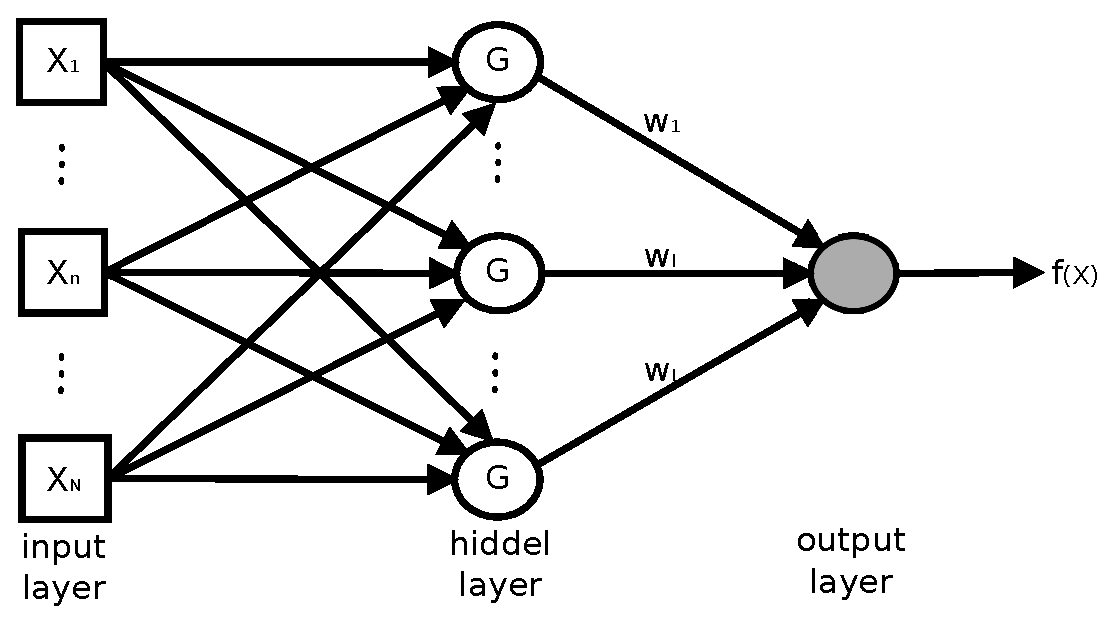
\includegraphics[width=90mm]{RBF.eps} 
\caption{Radial basis function network.}
\label{rbf1}
\end{figure}
The values that the radii or widths r take on may considerably affect the prediction abilities of the network; these are computed using heuristics,\cite{Haykin}. The output layer includes as many nodes as the responses of the network. The single response we are dealing with is expressed by the sum of the weighted output signals from the hidden neurons, as follows             
\begin{eqnarray}
	f(x)=\sum _1^N w_i*G(u(x_i),r)
\end{eqnarray}  



\section{Knowledge based systems (KBS)}
Knowledge-based systems are systems based on the methods and techniques 
of Artificial Intelligence. Their core components are the knowledge base and 
inference mechanisms. In this thesis a KBS that resembles Case-Based Reasoning (CBR) is in used.
CBR can be seen as a problem solving method that 
reuses past cases and experience to conceive a solution to a current problem. 
While other major artificial intelligence techniques rely on mapping generalized 
relationships between problem descriptions and conclusions. CBR has the benefit 
of utilizing previous experience based on concrete old-problem solutions. 
The central tasks of a CBR system to identify the problem in hand find one or 
more similar past case(s), use this information to suggest a solution to the current 
problem and update the system by learning from this experience \cite{kolodner_1991,kolodner_1993,slade_1991,riesbeck_1989}.      
%***********************************************************************

\paragraph{Historic note}
%***********************************************************************
\label{History} It is widely held that the origins of CBR lays in the work of 
Schank and Abelson in 1977 \cite{Schank_Abelson_1977}. They proposed that general 
human knowledge about situations is recorded as scripts that allows the extract 
of expectations and inferences. Scripts were proposed as structure for conceptual 
memory describing information about stereotypical events. However, experiments 
showed that they are not a complete theory of memory representation -people 
often confuse events with similar scripts. Such observations fell in line with 
concept formulation, problem solving and experimental learning theories within 
philosophy and psychology \cite{tulving_1977,smith_1978}. 

Roger Schank continued to investigate the role of previews situations (i.e. cases) 
and situation patterns role in both problem solving and learning \cite{Schank_1982}. 
Simultaneously Gentner \cite{genter_1983} was developing a also relevant to CBR 
theoretical framework for analogy. Significant references to CBR can also be fount in 
Wittgensteins's observation \cite{wittgestein_1953} that natural concepts are in fact 
polymorphic and can not be classified by a single set of necessary and sufficient 
features but instead can be defined by a set of instances (i.e. cases) with family 
resemblances. This work has been cited as the philosophical basis for CBR by Aamondt and Plaza \cite{aamond_plaza_1994}.

Whilst the philosophical roots of CBR could be claimed by many what is not in doubt 
is that it was Roger Schank and his group that in the early eighties produced both 
a cognitive model and the first CBR applications based on it. Janet Kolonder developed 
the first CBR system called CYRUS \cite{kolodner_1983a,kolodner_1983b} which was an 
implementation of Schank's dynamic memory model. Its case-memory model later served 
as the basis for several other CBR systems. Spreading there use in a lot of disciplines 
from law \cite{ashley_1988,rissland_skalak_1989} to civil engineering \cite{whatson_abdullah_1994,moore_1994}
%***********************************************************************
\subsection{Case-Based Reasoning}
%***********************************************************************
\label {CBR}  The classic definition of CBR was coined by Riesbeck and Schank \cite{riesbeck_1989}:

"A case-based reasoner solves problems by using or adapting solutions to old problems". 
Which answers exactly the what a CBR system should do but not the how it dose it. The answer 
to the second question is commonly described by the so called CBR-cycle (Fegure 1). 
%-----------------------------------------------------------------------
\paragraph{CBR Cycle}
%-----------------------------------------------------------------------
\label{CBR Cycle} CBR is based on four logical steps described by Aamodt and Plaza 
\cite{aamond_plaza_1994} as a typical cyclical process comprising the four REs: 

\begin{itemize}
  \item RETRIEVE the most similar case(s);
  \item REUSE the case(s) to attempt to solve the problem;
  \item REVISE the proposed solution if necessary, and
  \item RETAIN the new solution in the Case-Base.
\end{itemize}
which can be represented by a schematic cycle (see Figure \ref{cbr}).

\figuremacroW{cbr}{CBR}{Schematic cycle representing the four REs}{0.5}

%\begin{center}
%\begin{tabular}{ c }
%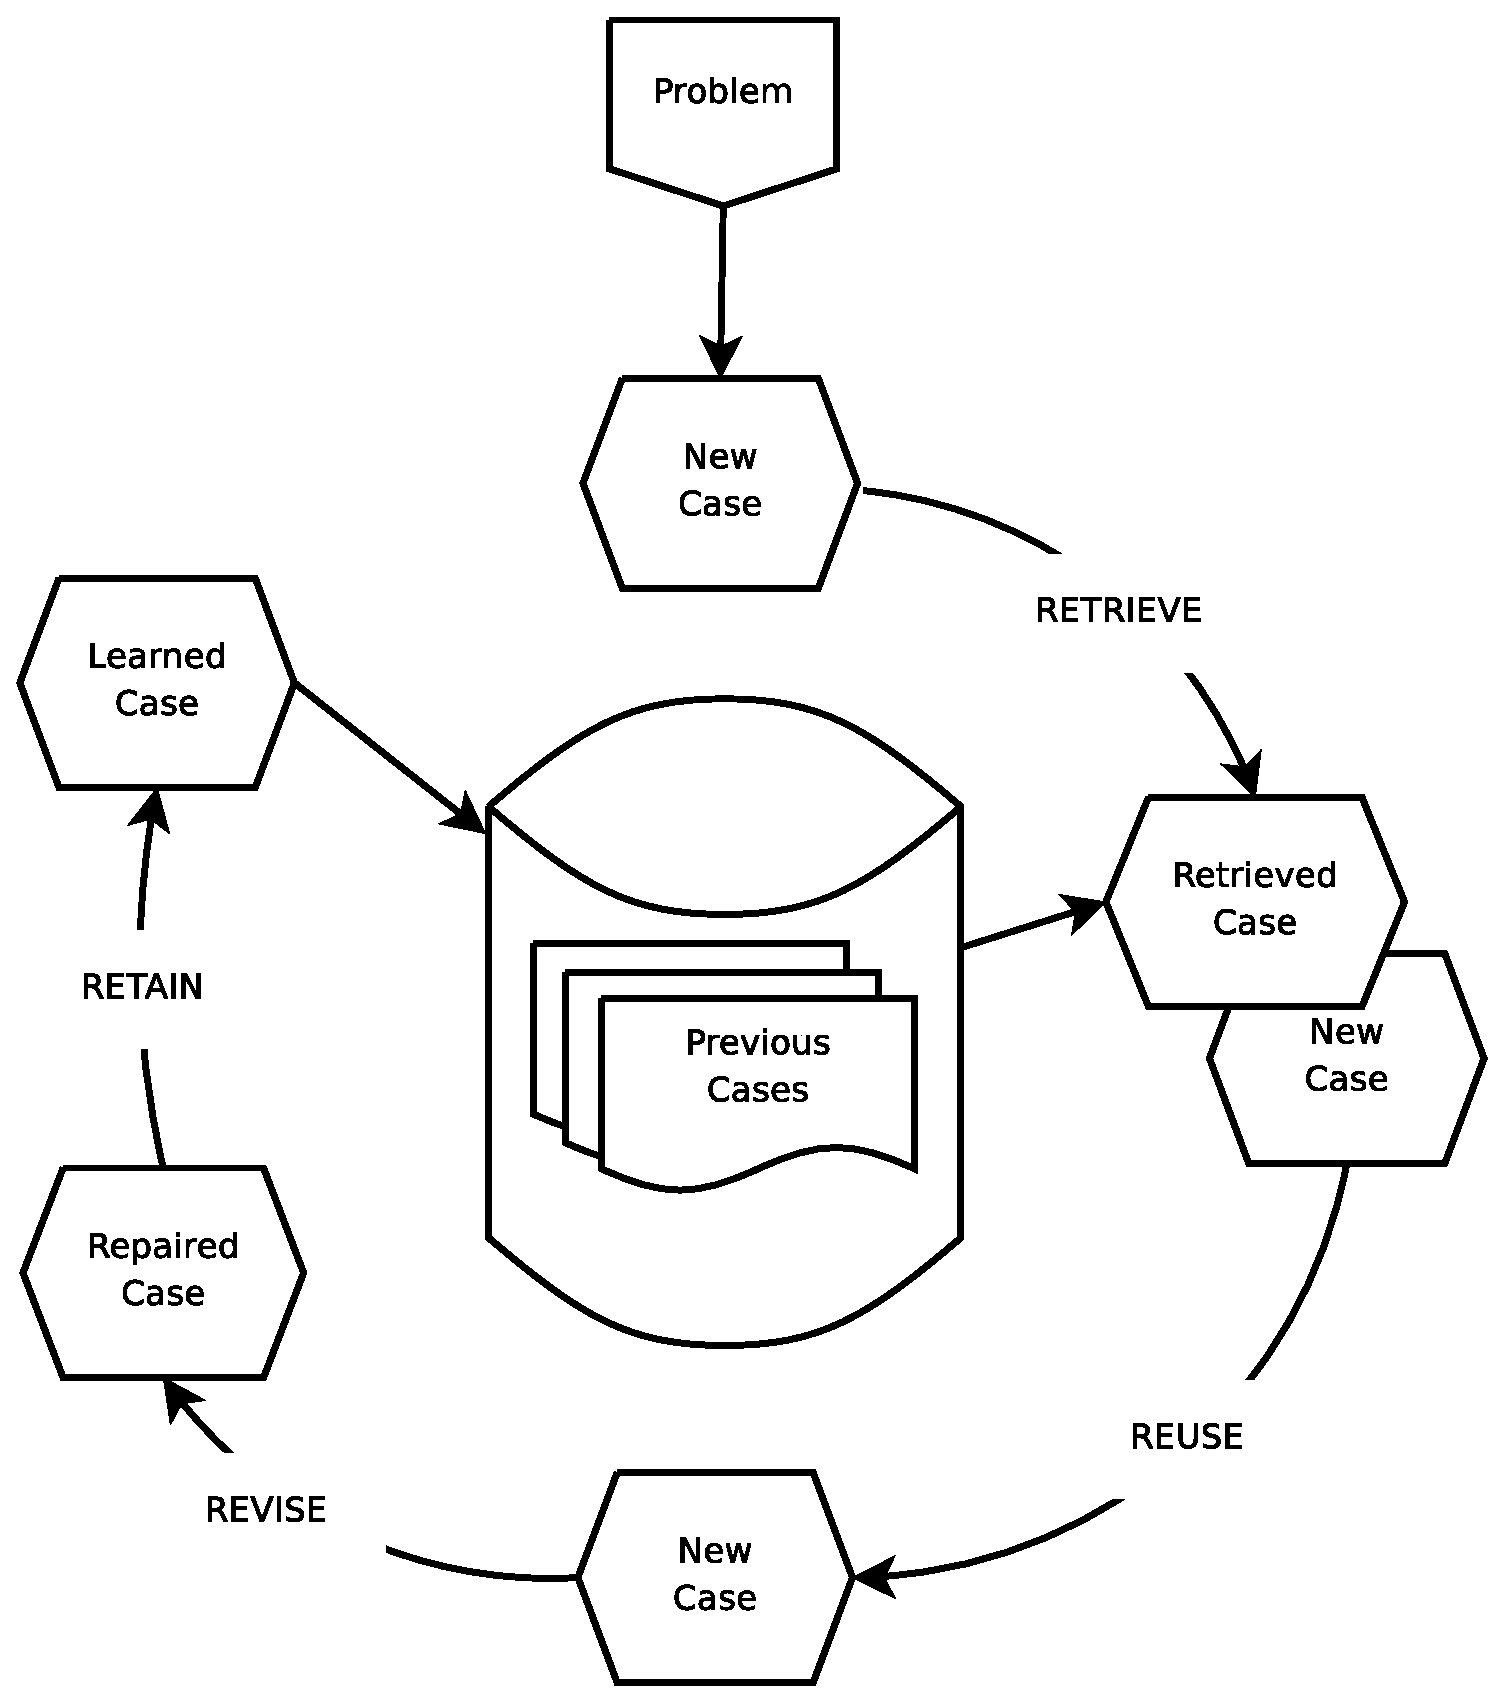
\includegraphics[width=70mm]{cbr.eps} \\
%Figure 1 Schematic cycle representing the four REs.
%\end{tabular}
%\end{center}

A new problem is matched against cases in the case base and thought a similarity 
criterion one or more similar cases are retrieved. A solution is suggested by the 
matching cases. Is then reused and tested for success. Unless the suggested solution 
is a close match it will probably have to be revised. In the end of this procedure the 
new case should be retained in the case-base. This cycle rarely is independent of 
human intervention. Many CBR tools act solely as case retrieval an reuse systems. 
Case revision (i.e. adaptation) is often left as a human task.   

The following sections will outline how each process in the cycle can be handled.

%-----------------------------------------------------------------------
\paragraph{Retrieve}
%-----------------------------------------------------------------------
\label{Retrieve} 
Given a description of a problem, a retrieval algorithm, using the indices in the case-memory, 
should retrieve the most similar case(s) to the current problem or situation. The retrieval algorithm 
relies on the indices and the organisation of the memory to direct the search to potentially useful cases.

The issue of choosing the best matching case has been addressed by research into analogy \cite{Falkenehainer_1986}. 
This approach involves using heuristics to constrain and direct the search. Several algorithms have 
been implemented to retrieve appropriate cases, for example: serial search 
\cite{Navinchandar_1991, Acorn_Walden_1992, Simoudis_93}, hierarchical search 
\cite{Maher_Zhang_1991} and simulated parallel search \cite{Domeshek_1993}.

Case-based reasoning will be ready for large scale problems only when retrieval algorithms
are efficient at handling thousands of cases. Unlike database searches that target a specific
 value in a record, retrieval of cases from the case-base must be equipped with heuristics 
that perform partial matches, since in general there is no existing case that exactly matches the new case.

Among well known methods for case retrieval are: nearest neighbour, induction, 
knowledge guided induction and template retrieval. These methods can be used 
alone or combined into hybrid retrieval strategies.

\subparagraph{Nearest neighbour}
\label{nearest neighbour}This approach involves the assessment of similarity 
between stored cases and the new input case, based on matching a weighted sum 
of features. The biggest problem here is to determine the weights of the features. 
The limitation of this approach include problems in converging on the 
correct solution and retrieval times. In general the use of this method leads 
to the retrieval time increasing linearly with the number of cases. Therefore 
this approach is more effective when the case base is relatively small. 

\subparagraph{Induction}
\label{Induction}Induction algorithms determine which features do the best job 
in discriminating cases, and generate a decision tree type structure to organise 
the cases in memory. This approach is useful when a single case feature is 
required as a solution, and where that case feature is dependent upon others.

\subparagraph{Knowledge guided induction}
\label{Knowledge guided induction} This method applies knowledge to the induction 
process by manually identifying case features that are known or thought to affect 
the primary case feature. This approach is frequently used in conjunction with other 
techniques, because the explanatory knowledge is not always readily available for large case bases.


\subparagraph{Template retrieval}
\label{template} Similar to SQL-like queries, template retrieval returns all 
cases that fit within certain parameters. This technique is often used before 
other techniques, such as nearest neighbour, to limit the search space to a 
relevant section of the case-base.

%-----------------------------------------------------------------------
\paragraph{Revise - Adaptation}
%-----------------------------------------------------------------------
\label{Revise} Once a solution is suggested based on the matching retrieved case(s) 
a CBR system should adapt the solution to the needs of the current case. Adaptation 
looks for prominent differences between the proposed solution and the current case and 
then applies formulae or rules that take those differences into account when 
suggesting an improved solution. In general, an ideal set of adaptation rules must be strong 
enough to generate complete solutions from scratch.

\subparagraph{}
Several techniques, ranging from simple to complex, have been used in CBR for adaptation. These include:

\textbf{Null adaptation,}a direct simple technique that applies whatever solution is retrieved to the current 
problem without adapting it. Null adaptation is useful for problems involving complex 
reasoning but with a simple solution. For example, when someone applies for a bank loan, 
after answering numerous questions the final answer is very simple: grant the loan, 
reject the loan, or refer the application.

\textbf{Parameter adjustment,}compares specified parameters of the retrieved 
and current case to modify the solution in an appropriate direction.

\textbf{Abstraction and respecialisation,}
a general adaptation technique that is used in a basic way to achieve simple 
adaptations and in a complex way to generate novel, creative solutions.

\textbf{Critic-based adaptation,}
in which a critic looks for combinations of features that can cause a problem in 
a solution. Importantly, the critic is aware of repairs for these problems.

\textbf{Reinstantiation,}
is used to instantiate features of an old solution with new features.

\textbf{Derivational replay,}
is the process of using the method of deriving an old solution or solution piece to derive a solution in the new situation.

\textbf{Model-guided repair,}
uses a causal model to guide adaptation.

\textbf{Case-based substitution,}
uses cases to suggest solution adaptation.
%-----------------------------------------------------------------------
\paragraph{Retain}
%-----------------------------------------------------------------------
\label{Retain} Case is a piece of knowledge representing an experience. This knowledge has to 
be retained in the case-base after a successful procedure \cite{kolodner_1993}. Typically a case comprises:   
\begin{itemize}
	\item the problem that describes the state of the world when the case occurred.
	\item the solution which states the derived solution to that problem.
	\item the outcome which describe the state of the world after the case occurred. 
\end{itemize}

There is a lack of consensus within the CBR community on what information should be in a case. However its advised that two measures can be taken into account when deciding,
 the functionality and the ease of acquisition of the information represented in the case \cite{kolodner_1993}. 
%%%%%%%%%%%%%%%%%%%%%%%%%%%%%%%%%%%%%%%%%%%%%%%%%%%%%%%%%%%%%%%%%%%%%%%%

%%%%%%%%%%%%%%%%%%%%%%%%%%%%%%%%%%%%%%%%%%%%%%%%%%%%%%%%%%%%%%%%%%%%%%%

\section{Knowledge based system assisted Evolutionary Algorithm}
In the design of fluid dynamic shapes a pattern of similar geometries typically occurs when dealing with similar problems.  
%Some may actually argue that all fluid dynamic shapes lookalike especially in comparison with non fluid dynamic ones. 
That fact turns the design of fluid dynamic shapes into an almost perfect candidate for the
use of CBR as a problem solving technique. 

In that case and due to the nature of the problem  
in hand, the design of a fluid dynamic shape with specific characteristics in a specific environment, 
the solution is always complex. Thus the need of adaptation (revise) is almost certain.  
\textit{Null adaptation is useful for problems involving complex
reasoning but with a simple solution.}

In order to have a fully automated system, the role of human intervention in adaptation has to be 
replaced by a set of adaptation rules. These rules take into account the derivations of the 
proposed solution compared to the desired one and suggest an improved proposal.
The rules that govern the evolution of species, ideally fit the above description. So an 
evolutionary algorithm (EA) is a perfect tool to undertake the revise step. 

Therefore the first of the new ideas presented in this thesis aims to extend the base optimization method (previews PhDs by LTT) by making it capable to accommodate and exploit pieces of useful information archived during previous relevant successful designs. So, instead of parameterizing the geometry of the hydraulic machine components, which inevitably leads to many design variables, enough to slow down the design procedure, in the proposed method all new designs are expressed as weighted combinations of the archived ones. The archived designs act as the design space base. The role of the optimization algorithms is to find the set (or sets, for more than one objectives, where the Pareto front of non-dominated solutions is sought) of weight values, corresponding to the hydraulic machine configuration(s) with optimal performance. Since the number of weights is much less that the number of design variables of the conventional shape parameterization, the design space dimension reduces and the CPU cost of the metamodel-assisted evolutionary algorithm is much lower.

\subsection{Designing a new component based on archived designs}
Let us assume that a small number of previous designs are available. These designs must have been performed for similar problems and archived with respect to all design variables, in conformity with the same parameterization. Let us denote by $GEO_i=(b_1^i,b_2^i,....,b_n^i)$, $i=1,m$ the m archived designs. Let $b_j (j=1,n)$ denote the “conventional” design variables. It is a simple matter to assume that any new design $b_j^{new} (j=1,n)$ may result from the combination of $m$ archived designs, by means of weights $w_i (i=1,m)$. This is, in fact, equivalent to a multi-linear interpolation scheme, namely:

\begin{eqnarray}
   b_j^{new} = \frac{\sum_{i=1}^{m}w_i \times b_j^i}{\sum_{i=1}^{m}w_i } 
   \label{linear} 
\end{eqnarray}

Without loss in generality, we may assume that $w_i \in [0,1]$. Setting up an optimization method merely based on eq.\ref{linear} leads to a parsimonious set of unknowns (or design variables, namely the m values of $w_i$; recall that m is a quite small number compared to n). However, since (a) m is small and (b) a multi-linear interpolation with the same weight for all variables comprising the same archived design is used, the flexibility and effectiveness of such a method is questionable. 

Among other, the set of the archived solutions reveals the statistical distribution of each design variable and, consequently, this can also be used to set the bounds of the design space. In place of eq.\ref{linear}, the nonlinear equations

\begin{eqnarray}
   b_j^{new} = \Phi _j^{-1} (\frac{\sum_{i=1}^{m}w_i \times \Phi _j(b_j^i)}{\sum_{i=1}^{m}w_i }) 
   \label{non-linear} 
\end{eqnarray}

can be used to define each new design. In eq.\ref{non-linear},$\Phi _j$ are appropriate nonlinear functions. Based on the assumption that the archived designs (which will otherwise be referred to as design bases) correspond to operating conditions correlated to the new ones, the new design should conform to a normal distribution. Should this be the case, the sigmoid cumulative distribution function could be used for $\Phi _j$  \cite{Kiemele}. 

\begin{eqnarray}
   \Phi _{\mu \sigma ^2} (x)= \frac{1}{\sigma\sqrt[2]{2\pi}}\int _{-\infty}^x exp(\frac{-(u-\mu)^2}{2 \sigma^2}) 
   \label{cdf} 
\end{eqnarray}

where $\mu$ (mean) and $\sigma$ (standard deviation) are calculated for each “conventional” design variable (j); schematically:

\begin{eqnarray}
		\left( {\begin{array}{c}
 		b_1^1  \\
 		\vdots  \\
 		b_n^1	\\
 		\end{array} } \right) 
 		\left( {\begin{array}{c}
 		b_1^i  \\
 		\vdots  \\
 		b_n^i	\\
 		\end{array} } \right)
 		\left( {\begin{array}{c}
 		b_1^m  \\
 		\vdots  \\
 		b_n^m	\\
 		\end{array} } \right) \rightarrow
		\left( {\begin{array}{c}
 		\mu _1  \\
 		\vdots  \\
 		\mu _n  \\
 		\end{array} } \right)
		\left( {\begin{array}{c}
 		\sigma _1  \\
 		\vdots  \\
 		\sigma _n  \\
 		\end{array} } \right)
   \label{cdf-matrix} 
\end{eqnarray}

The use of the cumulative distribution function, eq.\ref{cdf}, practically confines $b_i$ within $\mu _i \pm 3\sigma _i$. To overcome this limitation, a single extrapolation variable $\Psi$ which multiplies all computed (based on the archived designs) $\sigma$ values and, thus, extends the search space, is introduced. $\Psi$ is used as follows,


\begin{eqnarray}
		\left( {\begin{array}{c}
 		\sigma _1  \\
 		\vdots  \\
 		\sigma _n  \\
 		\end{array} } \right) =
 		\Psi \times 
 		\left( {\begin{array}{c}
 		\sigma _1^{computed}  \\
 		\vdots  \\
 		\sigma _n^{computed}  \\
 		\end{array} } \right)
   \label{cdf-matrix} 
\end{eqnarray}

With either eq.\ref{linear} or eq.\ref{non-linear}, an optimization problem with m weights (the number $m$ of design bases is considered to be small) as unknowns is neither effective nor flexible. Such a method may overcome the curse of dimensionality (since the number of design variables is no more depending on $n$) but may lead to sub-optimal solutions. For this reason, the grouping of design variables that correlate with each other must also be used. Correlated design variables such as, for instance, those defining the mean camber surface angle at LE, etc, are grouped together. After forming these groups, different weights are associated with each one of them. This is why the new weights are denoted by $w_{i,k}$, where the first index corresponds to the $i^{th}$ design basis and the second one to the $k^{th}$ group of design variables (which $b_i$ belongs to). In conclusion, in place of either eq.\ref{linear} or eq.\ref{non-linear}, the following equation


\begin{eqnarray}
   b_j^{new} = \Phi _j^{-1} (\frac{\sum_{i=1}^{m}w_{i,k} \times \Phi _j(b_j^i)}{\sum_{i=1}^{m}w_{i,k} }) 
   \label{non-linear2} 
\end{eqnarray}
is used. 

Based on eq.\ref{non-linear2}, an optimization problem with $m \times K$ unknowns (or $m\times K+1$, to also account for $\Psi$), where $K$ is the number of design variable groups, is set up. Search methods, such as EA (or MAEA), with the proposed parameterization may locate the global optimum, much more efficiently than an EA (or MAEA) based on the conventional parameterization. This is demonstrated within hydraulic turbo-machinery design/optimization cases further on. 

\figuremacroW{cbr_r}{Francis CBR}{Here a new Francis blade (light blue and yellow) is designed on the basis of 3 older ones (dark blue and red).}{0.7}

As an example the aforementioned technique the generation of a Francis blade as based on three similar (with respect of Q11 and N11) base blades is shown in fig.\ref{cbr_r}. The new design is the light blue and yellow one and is parameterized with 19 parameters ($3$ bases $\times 6$ groups $+1$ extrapolation parameter). The base designs are parameterized with 336 design variables each using a mean surface plus thickens parameterization (futher ditails about the parameterization are given in Chapter \ref{ParamEval})


% ---------------------------------------------------------------------------
% ----------------------- end of thesis sub-document ------------------------
% ---------------------------------------------------------------------------
